\documentclass[../TV&MS.tex]{subfiles}
\begin{document}
    
\section{Сходимость случайных величин}

\subsection{Виды сходимости}

	В этом разделе мы введем вагон непонятных определений, а потом постараемся 
	запутаться еще больше, доказывая, какая сходимость круче, и ковыряясь в контрпримерах. 
	Но для начала вспомним наших старых знакомых: измеримое пространство $(\Omega, \Ev)$, 
	вероятностное пространство $(\Omega, \Ev, \Pro)$ и случайную величину 
	$\xi \colon \Omega \rightarrow \Real$, которая обладает свойством
	$$\forall B \in \Bor \quad \xi^{-1}(B) = \{ \omega \in \Omega 
	\colon \xi(\omega) \in B \} \in \Ev.$$

	Пусть теперь $\xi, \xi_1, \xi_2, \dots$ "--- случайные величины на $(\Omega, \Ev)$.

\begin{Def}
	Последовательность случайных величин $\{\xi_n\}$ \mdef{сходится} к случайной величине 
	$\xi$ \mdef{почти наверное (с вероятностью 1)}, если вероятность множества тех 
	элементарных событий, где она не сходится, равно нулю.
	$$\{ \xi_n \} \xrightarrow{\text{п.н.}} \xi, \text{если} \quad 
	\Pro(\Set{\omega}{\xi_n(\omega) \nrightarrow \xi}) = 0.$$
\end{Def}

\begin{Ex}
	Пусть $\xi_n$ принимает значение $n$ в рациональных точках числовой прямой и $0$ "--- 
	в иррациональных. Тогда $\{\xi_n\} \xrightarrow{\text{п.н.}} 0$, так как мера множества 
	рациональных чисел, где случайная величина расходится, "--- ноль.
\end{Ex}

\begin{Def}
	Последовательность случайных величин $\{\xi_n\}$ \mdef{сходится} к случайной величине 
	$\xi$ \mdef{в среднем порядка $r$}, если $r$-ый момент их разности сходится к нулю.
	$$\{ \xi_n \} \xrightarrow{\text{(r)}} \xi, \text{если} \quad \Expec(\xi_n - \xi)^r 
	\xrightarrow[n \rightarrow +\infty]{} 0.$$
\end{Def}

\begin{Ex}
	Возьмем в качестве множества $\Omega$ окружность длины $1$, событиями будут борелевские 
	множества, а вероятность введем как меру Лебега. События $A_n$ введем таким образом: 
	$A_1$~"--- дуга длины $1/2$, отложенная от какой-то точки против часовой стрелки. 
	$A_n$~"--- дуга длины $\frac{1}{n+1}$, отложенная против часовой стрелки от конца 
	дуги $A_{n-1}$. Введем случайную величину: $\xi_n(\omega) = \Ind(\omega \in A_n)$
	Покажем, что $\{\xi_n\}$ сходится к $0$ в среднем любого положительного порядка.
	$$\Expec(\xi_n - \xi)^r = \Expec\xi_n^r = \Expec\left(\Ind(\omega \in A_n)\right)^r 
	= \Pro(A_n) = 1/n \xrightarrow[n \rightarrow +\infty]{} 0.$$
\end{Ex}

\begin{St}
	Из сходимости в среднем, вообще говоря, не следует сходимость почти наверное.
\end{St}

\begin{Proof}
	В рассмотренном выше примере $\xi_n(\omega)$ не сходится ни в одной точке окружности. 
	Действительно, так как ряд $\sum_{n=1}^\infty \frac{1}{n}$ расходится, то для любой 
	точки $\omega$ на окружности мы можем указать бесконечное число номеров $n_k$, 
	таких что $\omega~\in~A_{n_k}$.
\end{Proof}

\begin{St}
	Из сходимости почти наверное, вообще говоря, не следует сходимость в среднем.
\end{St}

\begin{Proof}
	Рассмотрим отрезок $[0, 1]$, с событиями, являющимися борелевскими множествами и 
	вероятностью, введенной как мера Лебега. Положим $\xi_n(\omega) = e^{n} 
	\Ind(\omega \in [0, 1/n])$. Тогда $\xi_n \xrightarrow{\text{п.н.}} 0$, но при этом 
	$\forall r > 0 \quad \Expec\xi_n^r = e^{np}\Expec\Ind(\omega \in [0, 1/n]) = e^{np}/n$, 
	а эта величина стремится к бесконечности, значит, сходимости в среднем нет.
\end{Proof}

	Введем еще один вид сходимости.

\begin{Def}
	Последовательность случайных величин $\{\xi_n\}$ \mdef{сходится} к случайной величине 
	$\xi$ \mdef{по вероятности}, если для любого сколь угодно малого положительного 
	$\varepsilon$ вероятность таких событий, что модуль разности $\xi_n$ и $\xi$ больше 
	$\varepsilon$, стремится к $0$.
	$$\{\xi_n\} \xrightarrow{\Pro} \xi, \text{если} \quad \forall \varepsilon > 0 \quad 
	\Pro(\Set{\omega}{|\xi_n(\omega) - \xi(\omega)| > \varepsilon}) 
	\xrightarrow[n \rightarrow +\infty]{} 0.$$
\end{Def}

\begin{Wtf}
	На этом моменте может немного поплавиться мозг в попытках понять, чем сходимость по 
	вероятности отличается от сходимости с вероятностью $1$. Действительно, и там и там мы 
	говорим, что вероятность тех событий, на которых случайная величина не сходится, равна 
	нулю. Но разница в том, что в случае сходимости почти наверное мы сначала устремляем $n$ 
	к бесконечности, а потом считаем вероятность, событий, когда не сходится, а в случае 
	сходимости по вероятности мы сначала посчитали вероятность для какого-то фиксированного 
	$n$, а потом устремились к бесконечности. 
\end{Wtf}

\begin{Ex}
	Докажем, что та жуткая последовательность случайных величин на окружности сходится 
	по вероятности к нулю. Действительно, 
	$$\Pro(\Set{\omega}{|\xi_n(\omega) - 0| > \varepsilon}) = \Pro(\Set{\omega}{\xi_n(\omega) 
	> \varepsilon}) = \Pro(\Set{\omega}{\xi_n(\omega) = 1}) = 
	1/n \xrightarrow[n \rightarrow +\infty]{} 0.$$
\end{Ex}

\begin{St}
	Только что рассмотренным примером мы доказали, что из сходимости по вероятности, 
	вообще говоря, не следует сходимость почти наверное.
\end{St}

\begin{St}
	Из сходимости по вероятности, вообще говоря, не следует сходимость в среднем.
\end{St}

\begin{Proof}
	Для доказательства воспользуемся примером про отрезок. Докажем, что 
	$\{\xi_n\} \xrightarrow{\Pro} 0$. Действительно, $\Pro{\Set{\omega}{\xi_n(\omega) > 
	\varepsilon}} = 1/n \xrightarrow[n \rightarrow +\infty]{} 0$. Отсутствие сходимости 
	в среднем мы уже доказали.
\end{Proof}

\begin{Th}
	Из сходимости почти наверное следует сходимость по вероятности.
\end{Th}

\begin{Proof}
	Сначала докажем, что $\{ \xi_n \} \xrightarrow{\text{п.н.}} \xi \quad 
	\Leftrightarrow \quad \Pro\left(\sup \limits_{k \geqslant n} |\xi_k -\xi| \geqslant 
	\varepsilon\right) \rightarrow 0$. Положим 
	$A_n^\varepsilon = \Set{\omega}{|\xi_n -\xi| \geqslant \varepsilon}$, 
	$A^\varepsilon = \varlimsup A_n^\varepsilon \equiv \bigcap\limits_{n=1}^\infty 
	\bigcup\limits_{k \geqslant n} A_k^\varepsilon$. Тогда:

	$$\Pro\left(\Set{\omega}{\xi_n(\omega) \nrightarrow \xi}\right) = 0 \quad 
	\Leftrightarrow \quad \Pro\left(\bigcup_{\varepsilon > 0} A^\varepsilon\right) = 0 
	\quad \Leftrightarrow \quad \Pro\left(\bigcup_{m=1} A^{1/m}\right) = 0 
	\quad \Leftrightarrow.$$
	
	$$\Leftrightarrow \quad \Pro(A^{1/m}) = 0, m \geqslant 1 \quad \Leftrightarrow \quad 
	\Pro(A^\varepsilon) = 0, \varepsilon > 0 \quad \Leftrightarrow \quad \Pro\left( 
	\bigcup_{k \geqslant n} A_k^\varepsilon \right) \xrightarrow[n \rightarrow \infty]{} 0, 
	\varepsilon > 0 \quad \Leftrightarrow.$$
	
	$$\Leftrightarrow \quad \Pro\left(\sup \limits_{k \geqslant n} |\xi_k -\xi| \geqslant 
	\varepsilon\right) \xrightarrow[n \rightarrow \infty]{} 0 \quad \Rightarrow \quad 
	\Pro\left( |\xi_k - \xi| \geqslant \varepsilon \right) \rightarrow 0.$$

	А последнее утверждение "--- это определение сходимости по вероятности.
\end{Proof}

\begin{Wtf}
	Совершенно жуткое доказательство, понимается методом вглядывания: если достаточно долго 
	медитировать над каждой импликацией, то все переходы в конце концов станут понятными.
\end{Wtf}

\begin{Th}
	Из сходимости в среднем следует сходимость по вероятности.
\end{Th}

\begin{Proof}
	Утверждение теоремы практически сразу же следует из обобщенного неравенства Чебышева:
	$$\Pro \left( |\xi_n - \xi| \geqslant \varepsilon \right) \leqslant 
	\frac{\Expec|\xi_n - \xi|^r}{\varepsilon^r}.$$

	Переходя в неравенстве к пределу при $n \rightarrow \infty$, получаем требуемое.
\end{Proof}

\begin{Def}
	Последовательность случайных величин $\{\xi_n\}$ \mdef{слабо сходится} к случайной 
	величине $\xi$, если для любой непрерывной и ограниченной функции последовательность 
	мат. ожиданий функций от $\xi_n$ сходится к мат. ожиданию функции от $\xi$.
	$$\{ \xi_n \} \xrightarrow{w} \xi, \text{если} \quad \forall f(x) \colon f(x) \in C \  
	\text{и} \  |f(x)| \leqslant M \quad \Expec{f(\xi_n)} \rightarrow \Expec{f(\xi)}.$$
\end{Def}

\begin{St}
	Из сходимости по вероятности следует слабая сходимость.
\end{St}

\begin{Proof}
	Пусть $f(x) \colon |f(x)| \leqslant M.$ Также $\forall \varepsilon > 0$ выберем $N$ так, 
	чтобы $\Pro{|\xi| > N} \leqslant \dfrac{\varepsilon}{4M}.$ Выберем $\delta$ так, чтобы 
	$\forall |x| \leqslant N$ и $|x - y| \leqslant \delta$ было выполнено неравенство 
	$|f(x) - f(y)| \leqslant \varepsilon/2$. Тогда:
\begin{multline*}
	\Expec{|f(\xi_n) - f(\xi)|} = \Expec{\left(|f(\xi_n) - f(\xi)|; |\xi_n - \xi| \leqslant 
	\delta; |\xi| \leqslant N\right)} + \\ \Expec{ \left( |f(\xi_n) - f(\xi)|; |\xi_n - \xi| 
	\leqslant \delta; |\xi| > N \right) } + \Expec{ \left( |f(\xi_n) - f(\xi)|; |\xi_n - \xi| 
	> \delta) \right) } \leqslant \\ \varepsilon/2 + \varepsilon/2 + 2M * \Pro(|\xi_n - \xi| 
	> \delta) = \varepsilon + \Pro(|\xi_n - \xi| > \delta).
\end{multline*}

	Но из сходимости по вероятности следует, что $\Pro(|\xi_n - \xi| > \delta) \rightarrow 0$, 
	значит при $n~\rightarrow~\infty \qquad \Pro(|\xi_n - \xi| > \delta) < \varepsilon$, 
	тогда $\Expec{|f(\xi_n) - f(\xi)|} < 2\varepsilon$, откуда в силу произвольного выбора 
	$\varepsilon$ и в силу того, что модуль числа не превосходит самого числа, получаем требуемое.
\end{Proof}


\begin{Def}
	Последовательность случайных величин $\{\xi_n\}$ \mdef{сходится} к случайной величине $\xi$ 
	\mdef{по распределению}, если функции распределения $\{\xi_n\}$ сходятся к функции 
	распределения $\xi$ во всех точках, в которых предельная функция распределения непрерывна.
	$$\{ \xi_n \} \xrightarrow{d} \xi, \text{если} \quad F_{\xi_n}(x) \rightarrow F_\xi 
	\quad \forall x \colon F_\xi(x) \in C(x).$$
\end{Def}

\begin{Ex}
	Пусть $\{ \xi_n \}$ принимает значения $0$ и $1 - \dfrac{1}{n}$ с вероятностями 
	$\dfrac{1}{2}$. Тогда функция распределения для случайной величины $\xi_i$ выглядит так 
	(Рис.~\ref{ris:distr_seq}): 

\begin{center}
\begin{minipage}{0.32\linewidth}
	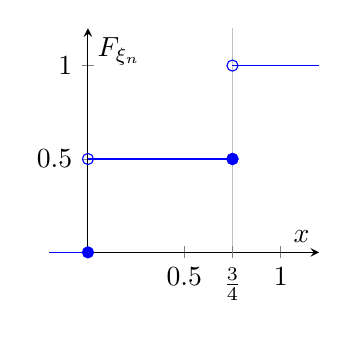
\begin{tikzpicture}
	\begin{axis}[
		scale=0.5,
		axis x line = middle,
		axis y line = middle,
		xlabel = {$x$},
		ylabel = {$F_{\xi_n}$},
		domain=-0.2:1.2
		ymin=-0.2,
		ymax=1.2,
		extra x ticks={0.75},
		extra x tick style={
			grid=major
		},
		extra x tick label={$\frac{3}{4}$}
	]
	\addplot[blue, domain=-0.2:0] {0};
	\addplot[blue, mark=*] coordinates {(0, 0)};
	\addplot[blue, mark=o] coordinates {
		(0, 0.5)
		(0.75, 0.5)
	};
	\addplot[blue, mark=*] coordinates {(0.75, 0.5)};
	\addplot[blue, mark=none, domain=0.75:1.2] {1};
	\addplot[blue, mark=o] coordinates {(0.75, 1)};
	\end{axis}
	\end{tikzpicture}
	\begin{center}
	\captionof{figure}{Функция \\ распределения $\xi_n$ \\ при $n = 4$}
	\end{center}	
	\label{ris:distr_seq}
\end{minipage}
\hspace{0.2cm}
\begin{minipage}{0.32\linewidth}
	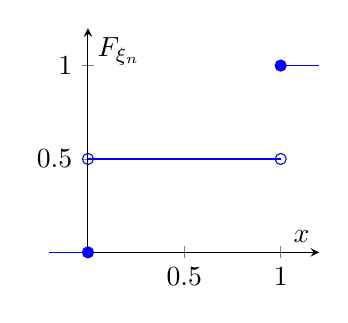
\begin{tikzpicture}
	\begin{axis}[
		scale=0.5,
		axis x line = middle,
		axis y line = middle,
		xlabel = {$x$},
		ylabel = {$F_{\xi_n}$},
		domain=-0.2:1.2
		ymin=-0.2,
		ymax=1.2
	]
	\addplot[blue, domain=-0.2:0] {0};
	\addplot[blue, mark=*] coordinates {(0, 0)};
	\addplot[blue, mark=o] coordinates {
		(0, 0.5)
		(1, 0.5)
	};
	\addplot[blue, mark=none, domain=1:1.2] {1};
	\addplot[blue, mark=*] coordinates {(1, 1)};
	\end{axis}
	\end{tikzpicture}
	\begin{center}
	\captionof{figure}{Предельная \\ функция}
	\end{center}
	\label{ris:limit_f}
\end{minipage}
\hspace{0.2cm}
\begin{minipage}{0.32\linewidth}
	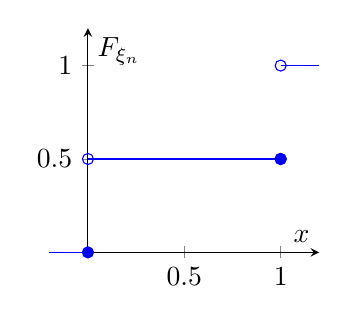
\begin{tikzpicture}
	\begin{axis}[
		scale=0.5,
		axis x line = middle,
		axis y line = middle,
		xlabel = {$x$},
		ylabel = {$F_{\xi_n}$},
		domain=-0.2:1.2
		ymin=-0.2,
		ymax=1.2
	]
	\addplot[blue, domain=-0.2:0] {0};
	\addplot[blue, mark=*] coordinates {(0, 0)};
	\addplot[blue, mark=o] coordinates {
		(0, 0.5)
		(1, 0.5)
	};
	\addplot[blue, mark=*] coordinates {(1, 0.5)};
	\addplot[blue, mark=none, domain=1:1.2] {1};
	\addplot[blue, mark=o] coordinates {(1, 1)};
	\end{axis}
\end{tikzpicture}
\begin{center}
\captionof{figure}{Функция \\ распределения $\xi$}
\end{center}
\label{ris:dist_lim}
\end{minipage}
\end{center}
\par\bigskip
	Тогда предельная функция будет выглядеть так (Рис.~\ref{ris:limit_f}). Заметим, 
	что она вообще не является функцией распределения, так как в точке $1$ нарушено 
	условие непрерывности слева. Тогда рассмотрим случайную величину $\xi$, 
	принимающую значение $0$ и $1$ с вероятностями $1/2$, тогда ее функция 
	распределения имеет вид (Рис.~\ref{ris:dist_lim}). Заметим, что предельная 
	функция и функция распределения $\xi$ различаются только в точке $1$, в которой 
	$F_\xi(x)$ не является непрерывной, значит $\{\xi_n\} \xrightarrow[]{d} \xi.$
\end{Ex}

\begin{St}
	Сходимость по распределению эквивалентна слабой сходимости.
\end{St}

\begin{Proof}
	\emph{\textbf{TODO:}} Чет я не знаю, как это доказать =(
\end{Proof}

\begin{St}
	Если последовательность случайных величин $\{ \xi_n \}$ сходится по распределению 
	к вырожденной случайной величине $\xi \xequiv{\text{п.н.}} a$, то $\{ \xi_n \}$ 
	сходится к $\xi$ по вероятности.
\end{St}

\begin{Proof}
	No.
\end{Proof}

	А теперь докажем теорему, ради которой мы и городили все эти огороды сходимостей. 
	Эта теорема впоследствии будет использоваться при доказательстве центральной 
	предельной теоремы.

\begin{Th}[теорема Леви о непрерывности]

\begin{enumerate}
	\item Пусть $\{ \xi_n \} \xrightarrow{d} \xi$ \ и \ $f_n(t) := \Expec e^{it\xi_n}$.
	Тогда $\{ f_n(t) \} \rightarrow f(t)$,\ где $f(t) = \Expec e^{it\xi}$.
	
	\item Пусть теперь $f_n(t) := \Expec e^{it\xi_n}$. Тогда если $f_n(t) \rightarrow 
	f(t) \quad \forall t \in \Real, \quad f(t) \in C(0)$, то $f(t)$ является 
	характеристической функцией некоторой случайной величины $\xi$, такой что 
	$\{ \xi_n \} \xrightarrow{d} \xi.$ 
\end{enumerate}
\end{Th}

\begin{Proof}
\begin{enumerate}
	\item Как было показано выше, сходимость по распределению эквивалентна слабой 
	сходимости. Положим в определении слабой сходимость функции $\varphi(x) := 
	Re(e^{itx})$ и $\psi(x) := Im(e^{itx})$, тогда $\Expec\varphi(\xi_n) \rightarrow 
	\Expec\varphi(\xi)$ и $\Expec\psi(\xi_n) \rightarrow \Expec\psi(\xi)$, откуда 
	следует утверждение теоремы.
	
	\item Ребята, не стоит вскрывать эту тему\ldots
\end{enumerate}
\end{Proof}

\begin{Wtf}
	А вот картинка, на которой схематично показано, что из чего следует.
\end{Wtf}

\begin{center}
\begin{tikzpicture}
	[
		st/.style={rectangle,draw}
	]
	\node[st] (prob1) {$\{ \xi_n \} \xrightarrow{\text{п.н.}} \xi$};
	\node[rectangle] (empty) [below=of prob1] {~};
	\node[st] (power) [below=of empty] {$\{ \xi_n \} \xrightarrow{(r)} \xi$};
	\node[st] (pro) [right=of empty] {$\{ \xi_n \} \xrightarrow{(\Pro)} \xi$};
	\node[st] (distr) [right=of pro] {$\{ \xi_n \} \xrightarrow{(d)} \xi$};
	\node[st] (weak) [below=of distr] {$\{ \xi_n \} \xrightarrow{(w)} \xi$};	
	\node (pn) at (3.8, -0.2) {$\xi \xequiv{\text{п.н.}} a$};
	\node[st] (th) [right=of distr] {т. о непрерывности};
	
	\draw [->] (prob1) -> (pro);
	\draw [->] (power) -> (pro);
	\draw [->] (pro) -> (distr);
	\draw [<->] (distr) -> (weak);
	\draw [->] (distr) to[bend right=45] (pro);
	\draw [dotted, line width=2pt] (distr) -> (th);
\end{tikzpicture}
\end{center}


\subsection{Закон больших чисел}
	В этой части рассмотрим закон больших чисел. Причем сначала скажем, как он 
	формулируется, а потом подсказываем его для различных исходных данных.

\begin{Def}
    Пусть $\{\xi_n\}$ "--- последовательность независимых одинаково распределенных 
    случайных величин, а $S_n = \sum\limits_{k=1}^{n} \xi_n$. Говорят, что 
    $\{\xi_n\}$ удовлетворяет \mdef{закону больших чисел (ЗБЧ)}, если 
    $\dfrac{S_n}{n} \xrightarrow[]{\Pro} \Expec \xi_i.$ 
\end{Def} 

\begin{Ex}
    Пусть $\xi_k$ независимы и равномерно распределены на отрезке $[-1, 1]$. 
    Тогда матожидание каждого слагаемого равно $0$. Тогда
\[
    \Pro \left( \left| \dfrac{S_n}{n} \right| \geqslant \varepsilon \right) 
    \leqslant \dfrac{\Disp S_n}{\varepsilon^2} = 
    \dfrac{\Disp \xi_1}{n \varepsilon^2} \rightarrow 0. 
\]
    То есть $\dfrac{S_n}{n}$ сходится по вероятности к своему матожиданию, 
    значит для данной последовательности случайных величин выполнен ЗБЧ.
\end{Ex} 

\begin{Th}[ЗБЧ в форме Хинчина]
    Если $\{ \xi_k \}$ "--- независимые одинаково распределенные случайные величины 
    с конечным матождиданием, то для них выполнен ЗБЧ. 
\end{Th} 

\begin{Proof}
    Первое желание, которое может возникнуть при виде данной теоремы"--- записать 
    неравенство Чебышева, но для неравенства Чебышева нужно не только конечное 
    матожидание, но и конечный второй момент, поэтому так не прокатит. Тогда мы 
    воспользуемся тем, что если последовательность случайных величин сходится к 
    числу, то сходимость по вероятности эквивалентна сходимости
    по распределению, и воспользуемся теоремой Леви о непрерывности.
\[
    f(t) := \Expec e^{it\xi_k} \quad \forall k=\overline{1 \ldots n}.  
\]

    Здесь нам не важно, для какой случайной величины считать харфункцию или 
    матожидание, так как они все одинаково распределены.
\[
    f_n(t) := \Expec e^{it\frac{S_n}{n}} = \Expec e^{it \frac{\xi_1 + \ldots + 
    \xi_n}{n}} = \prod\limits_{k=1}^{n} \Expec e^{\frac{it\xi_k}{n}} = 
    f^{n} \left( \frac{t}{n} \right).
\]

    Далее вспомним важной свойство харфункции: $a := f'(0) = \Expec \xi_k$. Тогда: 
\[
   	f^{n} \left( \dfrac{t}{n} \right) = \left( 1 + \dfrac{ita}{n} + \overline{o} 
   	\left( \dfrac{1}{n} \right)  \right)^{n} \xrightarrow[n \rightarrow \infty ]{} e^{ita}. 
\]

    Заметим, что $e^{ita}$ непрерывна на всей действительной прямой и обращается в $1$ 
    при $t = 0$. Значит по теореме о непрерывности $e^{ita}$ представляет собой харфункцию 
    некоторой случайной величины, к которой сходится по распределению $\dfrac{S_n}{n}$. 
    Действительно, эта случайная величина $\xi \xequiv{\text{п.н.}} a$.
    Таким образом, имеем, что $\dfrac{s_n}{n} \xrightarrow[]{w} \Expec \xi_k$,
    но если предельная случайная величина вырождена, то сходимость по распределению 
    эквивалентна сходимости по вероятности, значит 
    $\dfrac{s_n}{n} \xrightarrow[]{\Pro} \Expec \xi_k$.
\end{Proof} 

	Лулзов ради закинем еще парочку ЗБЧ.

\begin{Th}[ЗБЧ в форме Чебышева]
    Пусть $\{ \xi_k \}$ "--- последовательность не\-коррелированных случайных величин 
    с равномерно ограниченной дисперсией. То есть $\sup\limits_{k \in \mathbb{N}} 
    \Disp \xi_k \leqslant C < \infty$. Тогда для данной последовательности случайных 
    величин выполнен ЗБЧ.
\end{Th}

\begin{Proof}
    Последовательно воспользуемся неравенством Чебышева, некоррелированостью случайных 
    величин (а значит дисперсия суммы равна сумме дисперсий) 
    и равномерной ограниченностью дисперсий.
\[
    \Pro \left( \left| \dfrac{S_n}{n} - \Expec \xi_k \right| \geqslant \varepsilon \right) = 
    \Pro \left( \left| \dfrac{S_n - \Expec S_n}{n} \right| \geqslant \varepsilon \right) 
    \leqslant \dfrac{\Disp S_n}{(n\varepsilon)^2} =
    \dfrac{1}{n^2\varepsilon^2} \sum\limits_{k=1}^{n} \Disp \xi_k \leqslant
    \dfrac{C}{n\varepsilon^2} \xrightarrow[n \rightarrow \infty]{} 0.
\] 
\end{Proof} 

\begin{Note}
    Условия теоремы можно ослабить: вместо некоррелированности потребовать, чтобы сумма 
    ковариаций обращалась в 0, а вместо равномерной ограниченности константой можно 
    потребовать, чтобы дисперсии росли строго медленнее, чем линейная функция.
\end{Note} 

\begin{Th}[Усиленный ЗБЧ (УЗБЧ) в форме Колмогорова]
    Если $\{ \xi_k \}$ "--- независимые одинаково распределенные случайные величины с 
    конечным матождиданием, то $\dfrac{S_n}{n} \xrightarrow[]{\text{п.н.}}  \Expec \xi_k$. 
\end{Th}

\begin{Note}
    Условия те же, что и на ЗБЧ в форме Хинчина, но сходимость уже не по вероятности, 
    а почти наверное.
\end{Note} 

\begin{Proof}
    Все верно. Отвечаю.
\end{Proof} 

\begin{Wtf}
    Собственно, а к чему будут сходиться средние арифметические, если нет матожидания?
\end{Wtf} 

\begin{Ex}
    Распределим $\{ \xi_k \}$ по Коши с параметрами $C(0, \gamma)$ и посмотрим, 
    что будет происходить со средними арифмитическими.
\[
    p_{\xi_k} (x) = \dfrac{1}{\pi \gamma \left( 1 + \left( \dfrac{x}{\gamma} 
    \right)^2 \right) }, \quad f(t) :=  \Expec e^{it\xi_k} = e^{-\gamma \left| t \right| }.
\]

\begin{multline*}
    f_n(t) := \Expec S_n = \Expec e^{it \sum\limits_{k=1}^{n} \xi_k} = 
    \prod\limits_{k=1}^{n} \Expec e^{it\xi_k} = f^{n} \left( t \right) =
    e^{-\gamma n \left| t \right| } \implies \\
    p_{S_n} \left( t \right) = \dfrac{1}{\pi n \gamma \left( 1 + \left( 
    \dfrac{x}{n \gamma} \right)^2 \right) }.
\end{multline*}
    
    Теперь предположим, что последовательность $\{ S_n \} $ сходится по вероятности к 
    чему-то, и придем к противоречию. Пусть $\Pro \left( \left| \dfrac{S_n}{n} - a \right| 
    \geqslant \varepsilon \right) \rightarrow 0$. Тогда:
\begin{multline*}
	\Pro \left( \left| \dfrac{S_n}{n} - a \right| \geqslant \varepsilon \right) = 
	\int\limits_{n(a+\varepsilon)}^{+\infty} p(x)dx + \int\limits_{-\infty}^{n(a - 
	\varepsilon)} p(x)dx = \dfrac{1}{\pi} \left. \arctg \left( \dfrac{x}{\gamma n} \right) 
	\right|_{n(a+\varepsilon)}^{+\infty} + \dfrac{1}{\pi} \left. \arctg \left( 
	\dfrac{x}{\gamma n} \right) \right|_{-\infty}^{n(a - \varepsilon)} = \\
    = \dfrac{1}{\pi} \left( \arctg \left( \dfrac{a - \varepsilon}{\gamma} \right) - 
    \arctg \left( \dfrac{a + \varepsilon}{\gamma} \right)  \right) 
    \xcancel{ \xrightarrow[n \rightarrow \infty]{}} \ 0.
\end{multline*}
    Таким образом, последовательность средних арифметических случайных величин, 
    распределенных по Коши, не сходится по вероятности вообще ни к чему.
\end{Ex} 

\subsection{Центральная предельная теорема}

	С места в карьер:

\begin{Def}
    Последовательность случайных величин $\{ \xi_k \}$ \mdef{удовлетворяет ЦПТ}, 
    если $\exists \{ a_k \} \in \Real, \{ b_k \} > 0$, такие что 
\[
    \dfrac{S_k - a_k}{b_k} \xrightarrow[]{d} \xi \sim \Norm(0, 1).
\] 
\end{Def}

	Разомнемся на чем-нибудь попроще.

\begin{Th}
    Пусть $\{ \xi_k \}$ "--- норсв с конечным матожиданием и конечной ненулевой 
    дисперсией. Тогда $\{ \xi_k \}$ удовлетворяет ЦПТ, причем $a_n = \Expec S_n$,
    a $b_n = \sqrt{\Disp S_n}$, где  $S_n = \sum\limits_{k=1}^{n} \xi_k$.
\end{Th}

\begin{Note}
    Здесь распределение $\dfrac{S_k - \Expec \xi_k}{\sqrt{\Disp \xi_k}}$ сходится к 
    стандартному нормальному не абы как, а очень даже равномерно по $x$ на всей 
    действительной прямой.
\end{Note} 

\begin{Proof}
    Без ограничения общности будем считать, что $\Expec\xi_k=0$ и  $\Disp \xi_k = 1$.
    Тогда 
\[
    f(t) := \Expec e^{it\xi_k} = 1 + \cancelto{\text{\scriptsize{0}}}{ita} 
    \quad - \dfrac{t^2}{2} + \overline{o} \left( \dfrac{1}{n} \right). 
\]
    
\[
    f_{\frac{S_n}{\sqrt{n}}} (t) = \Expec e^{it\frac{S_n}{\sqrt{n}}} = 
    \left( f \left( \dfrac{t}{\sqrt{n}} \right) \right)^{n} = 
    \left( 1 - \dfrac{t^2}{2n} + \overline{o} \left( \dfrac{1}{n} \right)  \right)^{n} 
	\xrightarrow[n \rightarrow \infty]{} e^{-\frac{t^2}{2}}.
\] 

    Таким образом, харфункция центрированной нормированной случайной величины сходится 
    слабо к харфункции стандартного нормального распределения, а значит, центрированная 
    нормированная случайная величина сходится по распределению к $\Norm(0, 1)$.
\end{Proof} 

\begin{Why}
    Если вам уже стало плохо, то переживать не стоит "--- дальше будет еще хуже
\end{Why} 

	С этого момента положим:
\begin{itemize}
    \item Случайные величины $\{ \xi_k \}$ независимы и определены на 
    одном вероятностном пространстве.

    \item $F_k(x) = \Pro (\xi_k < x)$.
    \item $S_n = \sum\limits_{k=1}^{n} \xi_k$.
    \item $a_k = \Expec \xi_k$, $A_n = \sum\limits_{k=1}^{n} a_k$. 
    \item $b_k^2 = \Disp \xi_k$, $B_n^2 = \sum\limits_{k=1}^{n} b_k^2$.
\end{itemize} 

\begin{Th}[Ляпунова]
    Пусть $\mu_k^3 := \Expec \left| \xi_k - a_k \right|^3 < \infty, \quad
    M_n^3 := \sum\limits_{k=1}^{n} \mu_k^3$. Пусть выполнено 
    \emph{условие Ляпунова}:
\begin{equation}\label{Lyapunov}
    \dfrac{M_n^3}{B_n^3} \xrightarrow[n \rightarrow \infty]{} 0
\end{equation}
    
    Тогда $\{ \xi_k \}$ удовлетворяет ЦПТ.
\end{Th}

\begin{Th}[Линдеберга]
    Пусть $\varepsilon > 0$. Тогда если  $a_k < \infty$, $b_k < \infty$ и 
    выполнено \emph{условие Линдеберга}:
\begin{equation}\label{Lindeberg}
	L_n(\varepsilon) = \dfrac{1}{B_n^2} \sum\limits_{k=1}^{n} 
    \int\limits_{ \left| x - a_k \right| > \varepsilon B_n}^{}
	\left( x - a_k \right)^2 dF_k(x) \xrightarrow[n \rightarrow \infty]{} 0,
\end{equation} 

    То $\{ \xi_k \}$ удовлетворяет ЦПТ.
\end{Th} 

\begin{Note}
    Если случайные величины одинаково распределены, то условие Линдеберга 
    эквивалентно существованию дисперсии.
\end{Note}

\begin{Def}
    $\{ \xi_k \} $ удовлетворяют \mdef{условию Феллера}, если
\begin{equation}\label{Feller}
	\forall \varepsilon > 0 \quad
    \max\limits_{1 \leqslant k \leqslant n}
	\Pro \left( \dfrac{ \left| \xi_k - a_k \right| }{B_n} \right) > \varepsilon
    \xrightarrow[n \rightarrow \infty]{} 0. 
\end{equation}
\end{Def} 

\begin{Th}
\[
    \begin{cases}
        \text{ЦПТ} \\
        \eqref{Feller}
    \end{cases}
    \iff \eqref{Lindeberg}.
\]
\end{Th} 

\begin{Proof}
    Покажем, что из (\ref{Lindeberg}) следует (\ref{Feller}).
\[    
    \max_{1 \leqslant k \leqslant n} \Pro \left( \frac{ \left| \xi_k - 
    a_k \right|}{B_n} > \varepsilon \right) \leqslant \max_{1 \leqslant k 
    \leqslant n} \frac{b_k^2}{\varepsilon^2 B_n^2} = \max_{1 \leqslant k 
    \leqslant n} \frac{b_k^2}{\varepsilon^2 \left( b_1^2 +  \ldots + b_n^2 \right) }.
\]

\begin{multline*}
	\max_{1 \leqslant k \leqslant n} \Pro \left( \left| \xi_k - a_k \right| > 
	\varepsilon B_n \right)\leqslant\sum\limits_{k=1}^{n} \Pro \left( \left| 
	\xi_k - a_k \right| > \varepsilon B_n \right)=\sum\limits_{k=1}^{n} 
	\int\limits_{ \left| x - a_k \right| > \varepsilon B_n}^{} 1 dF_k(x) = \\
    \sum\limits_{k=1}^{n} \int\limits_{ \left| x - a_k \right| > \varepsilon B_n}^{} 
    \frac{(x - a_k)^2}{(x - a_k)^2} dF_k(x) \leqslant \frac{1}{\varepsilon^2 B_n^2} 
    \int\limits_{ \left| x - a_k \right| > \varepsilon B_n}^{} (x - a_k)^2 dF_k(x) 
    \xrightarrow[n \rightarrow \infty]{} 0.
\end{multline*} 

    Таким образом, условие Линдеберга влечет за собой условие Феллера.
\end{Proof} 

\begin{Th}
    Условие Ляпунова (\ref{Lyapunov}) влечет за собой условие Линдеберга (\ref{Lindeberg}).
\end{Th}

\begin{Proof}
\begin{multline*}
	L_n(\varepsilon) = \frac{1}{B_n^2} \sum\limits_{k=1}^{n}  
	\int\limits_{ \left| x - a_k \right| > \varepsilon B_n}^{} (x - a_k)^2 dF_k(x) = 
    \frac{1}{B_n^2} \sum\limits_{k=1}^{n} \int\limits_{ \left| x - a_k \right| > 
    \varepsilon B_n}^{} \frac{|x - a_k|^3}{|x - a_k|} dF_k(x) \leqslant\\
    \leqslant \frac{1}{\varepsilon B_n^3} \sum\limits_{k=1}^{n} 
    \int\limits_{-\infty}^{+\infty} \left| x - a_k \right|^3 dF_k(x) = 
    \frac{M_n^3}{\varepsilon B_n^3} \xrightarrow[n \rightarrow \infty]{} 0.
\end{multline*}
\end{Proof} 

\begin{Th}[Неравенство Берри"--~Эссена]
    $\sup\limits_{x} \left| \Pro \left( \dfrac{S_n - A_n}{B_n} < x \right) - 
    \Phi(x) \right| \leqslant C\dfrac{M_n^3}{B_n^3}$.

    Если случайные величины одинаково распределены, то правую часть можно переписать так:
\[
    C \frac{M_n^3}{B_n^3} = C_0 \frac{n \mu_k^3}{n^{3/2} b_k^3} =
    C_0 \frac{\mu_k^3}{b_k^3 \sqrt{n}}.
\] 
    Константу $C_0$ уточняли, уточняли, уточняли и в конце концов доуточнялись до 
    $C_0 \geqslant \dfrac{\sqrt{10} + 3}{6 \sqrt{2 \pi}}$. А потом доказали, 
    что здесь вообще стоит строгое равенство.
\end{Th}

\newpage



\end{document}
